\pdfminorversion=4 % for acroread
\ifdefined\ishandout
  \documentclass[aspectratio=169,t,handout,xcolor={usenames,dvipsnames}]{beamer}
\else
  \documentclass[aspectratio=169,t,xcolor={usenames,dvipsnames}]{beamer}
\fi

\usepackage{../beamerstyle}
\usepackage{dsfont}
\usepackage{bm}
\usepackage[english]{babel}
\usepackage[utf8]{inputenc}
\usepackage{graphicx}
\usepackage{algorithm}
\usepackage[ruled,vlined,algo2e,linesnumbered]{algorithm2e}
%\usepackage[boxed,vlined]{algorithm2e}
\usepackage{hyperref}
\usepackage{booktabs}
\usepackage{mathtools}

\usepackage{amsmath,amssymb}
\usepackage{listings}
\lstset{frame=lines,framesep=3pt,numbers=left,numberblanklines=false,basicstyle=\ttfamily\small}

\usepackage{subfig}
\usepackage{multicol}
%\usepackage{appendixnumberbeamer}
%
\usepackage{tcolorbox}

\usepackage{pgfplots}
\usepackage{tikz}
\usetikzlibrary{trees} 
\usetikzlibrary{shapes.geometric}
\usetikzlibrary{positioning,shapes,shadows,arrows,calc,mindmap}
\usetikzlibrary{positioning,fadings,through}
\usetikzlibrary{decorations.pathreplacing}
\usetikzlibrary{intersections}
\usetikzlibrary{positioning,fit,calc,shadows,backgrounds}
\pgfdeclarelayer{background}
\pgfdeclarelayer{foreground}
\pgfsetlayers{background,main,foreground}
\tikzstyle{activity}=[rectangle, draw=black, rounded corners, text centered, text width=8em]
\tikzstyle{data}=[rectangle, draw=black, text centered, text width=8em]
\tikzstyle{myarrow}=[->, thick, draw=black]

% Define the layers to draw the diagram
\pgfdeclarelayer{background}
\pgfdeclarelayer{foreground}
\pgfsetlayers{background,main,foreground}

%\usepackage{listings}
%\lstset{numbers=left,
%  showstringspaces=false,
%  frame={tb},
%  captionpos=b,
%  lineskip=0pt,
%  basicstyle=\ttfamily,
%%  extendedchars=true,
%  stepnumber=1,
%  numberstyle=\small,
%  xleftmargin=1em,
%  breaklines
%}

 
\definecolor{blue}{RGB}{0, 74, 153}

\usetheme{Boadilla}
%\useinnertheme{rectangles}
\usecolortheme{whale}
\setbeamercolor{alerted text}{fg=blue}
\useoutertheme{infolines}
\setbeamertemplate{navigation symbols}{\vspace{-5pt}} % to lower the logo
\setbeamercolor{date in head/foot}{bg=white} % blue
\setbeamercolor{date in head/foot}{fg=blue}
\setbeamercolor{author  in head/foot}{bg=white} %blue
\setbeamercolor{title in head/foot}{bg=white} % blue
\setbeamercolor{title}{fg=white, bg=blue}
\setbeamercolor{block title}{fg=white,bg=blue}
\setbeamercolor{block body}{bg=blue!10}
\setbeamercolor{frametitle}{fg=white, bg=blue}
\setbeamercovered{invisible}

% \makeatletter
% \setbeamertemplate{footline}
% {
%   \leavevmode%
%   \hbox{%
%   \begin{beamercolorbox}[wd=.333333\paperwidth,ht=2.25ex,dp=1ex,center]{author in head/foot}%
% %    \usebeamerfont{author in head/foot}\insertshortauthor
%   \end{beamercolorbox}%
%   \begin{beamercolorbox}[wd=.333333\paperwidth,ht=2.25ex,dp=1ex,center]{title in head/foot}%
%     \usebeamerfont{title in head/foot}\insertshorttitle
%   \end{beamercolorbox}%
%   \begin{beamercolorbox}[wd=.333333\paperwidth,ht=2.25ex,dp=1ex,right]{date in head/foot}%
%     \usebeamerfont{date in head/foot}\insertshortdate{}\hspace*{2em}
% %    \insertframenumber\hspace*{2ex} 
%   \end{beamercolorbox}}%
%   \vskip0pt%
% }
% \makeatother

%\pgfdeclareimage[height=1.2cm]{automl}{images/logos/automl.png}
%\pgfdeclareimage[height=1.2cm]{freiburg}{images/logos/freiburg}

%\logo{\pgfuseimage{freiburg}}

\renewcommand{\comment}[1]{
	\noindent
	%\vspace{0.25cm}
	{\color{red}{\textbf{TODO:} #1}}
	%\vspace{0.25cm}
}
\newcommand{\notefh}[1]{\textcolor{red}{\textbf{FH:} #1}}
\renewcommand{\comment}[1]{}
\newcommand{\hide}[1]{}
\newcommand{\cemph}[2]{\emph{\textcolor{#1}{#2}}}

\newcommand{\lit}[1]{{\footnotesize\color{black!60}[#1]}}

\newcommand{\litw}[1]{{\footnotesize\color{blue!20}[#1]}}


\newcommand{\myframe}[2]{\begin{frame}[c]{#1}#2\end{frame}}
\newcommand{\myframetop}[2]{\begin{frame}{#1}#2\end{frame}}
\newcommand{\myit}[1]{\begin{itemize}#1\end{itemize}}
\newcommand{\myblock}[2]{\begin{block}{#1}#2\end{block}}


\newcommand{\votepurple}[1]{\textcolor{Purple}{$\bigstar$}}
\newcommand{\voteyellow}[1]{\textcolor{Goldenrod}{$\bigstar$}}
\newcommand{\voteblue}[1]{\textcolor{RoyalBlue}{$\bigstar$}}
\newcommand{\votepink}[1]{\textcolor{Pink}{$\bigstar$}}

\newcommand{\diff}{\mathop{}\!\mathrm{d}}
\newcommand{\refstyle}[1]{{\small{\textcolor{gray}{#1}}}}
\newcommand{\hands}[0]{\includegraphics[height=1.5em]{images/hands}}
\newcommand{\transpose}[0]{{\textrm{\tiny{\sf{T}}}}}
\newcommand{\norm}{{\mathcal{N}}}
\newcommand{\cutoff}[0]{\kappa}
\newcommand{\instD}[0]{\dataset}
\newcommand{\insts}[0]{\mathcal{I}}
\newcommand{\inst}[0]{i}
\newcommand{\instI}[1]{i^{(#1)}}

% Iteration specific instance of variable/function/anything
% Introduced in the BO section, but moved up here to make it available within other macros
\newcommand{\iter}[2][\bocount]{{#2}^{(#1)}}

%--------HPO parameter macros-----------

% Parameter Configuration Space
\newcommand{\pcs}[0]{\pmb{\Lambda}}

% ???
\newcommand{\bx}[0]{\conf}

% Parameter Configuration
\newcommand{\conf}[0]{\pmb{\lambda}}

% Final Configuration
\newcommand{\finconf}[0]{\pmb{\hat{\lambda}}}

% Configuration corresponding to a given iteration -- better use \iter!
\newcommand{\confI}[1]{{\conf}^{(#1)}}

% Default Configuration
\newcommand{\defconf}[0]{{\conf}_{\text{def}}}

% Incumbent Configuration
\newcommand{\incumbent}[1][\bocount]{\iter[#1]{\finconf}}

% Optimal Configuration
\newcommand{\optconf}[0]{{\conf}^*}

% Configuration Space
\newcommand{\confs}[0]{\pcs}

%----------------------------------------

%\newcommand{\vlambda}[0]{\bm{\lambda}}
%\newcommand{\vLambda}[0]{\bm{\Lambda}}
\newcommand{\dataset}[0]{\mathcal{D}}
\newcommand{\datasets}[0]{\mathbf{D}}
\newcommand{\loss}[0]{L}
\newcommand{\risk}{\mathcal{R}}
\newcommand{\riske}{\mathcal{R}_{\text{emp}}}
\newcommand{\cost}[0]{c}
\newcommand{\costI}[1]{c^{(#1)}}

% Gaussian Process
\newcommand{\gp}{\mathcal{G}}
% Family of Objective Functions
\newcommand{\objF}{F}

%---------------BO Macros------------------

% BO loop counter
\newcommand{\bocount}{t}
% BO loop counter max, the counter runs from 1 to this value
\newcommand{\bobudget}{T}
% BO loop observation
\newcommand{\obs}[1][\conf]{\cost({#1})}
% BO loop observation space
\newcommand{\obsspace}{\mathcal{Y}}
% BO loop next observation
\newcommand{\bonextobs}{\obs[\iter{\conf}]}
% Acquisition Function, no args
\newcommand{\acq}{u}
% Standard Normal PDF
\newcommand{\pdf}{\phi}
% Standard Normal CDF
\newcommand{\cdf}{\Phi}
% Mean
\newcommand{\mean}{\mu}
% Standard Deviation
\newcommand{\stddev}{\sigma}
% Variance
\newcommand{\variance}{\sigma^2}
% Noise
\newcommand{\noise}{\nu}
% BO loop next selected sample
\newcommand{\bonextsample}{\confI{\bocount}}

% Single hyperparameter
\newcommand{\hyperparam}{\lambda}

% Single hyperparameter within a hyperparameter configuration
\newcommand{\hyperparami}[1][i]{{\hyperparam}_#1}

% Full definition of final configuration
\newcommand{\finconffull}{\incumbent[\bobudget]}

% Dataset
\newcommand{\datasetHPO}{{\dataset}_{HPO}}

% Dataset definition
\newcommand{\datasetHPOdef}{{\langle \bonextsample,\,\bonextobs \rangle}_{\bocount=1}^{\bobudget}}

% Double Display Fraction, forces large displays for everything in numerator and denominator
\newcommand\ddfrac[2]{\frac{\displaystyle #1}{\displaystyle #2}}

% Conditional Probability "Given That" Relation, source:https://tex.stackexchange.com/a/141685/205886
\newcommand\given[1][]{\:#1\vert\:}

% Expectation as a math operator
\DeclareMathOperator*{\E}{\mathbb{E}}

% Citation 
\newcommand{\source}[1]{
    \begin{flushright}
    	Source: \lit{#1}
    \end{flushright}
}
%-------------------------------------------

%Real numbers set
\newcommand{\realnum}{\mathbb{R}}
%Configuration space - do not use
%\newcommand{\configspace}{\Theta}
%Instances - do not use
%\newcommand{\instances}{\mathcal{I}}
%Expected value
\newcommand{\expectation}{\mathbb{E}}
%Kernel
\newcommand{\kernel}{\kappa}
%Constraint function
\newcommand{\constraintf}{c}
%Normal distribution
\newcommand{\normaldist}{\mathcal{N}}

% \renewcommand{\vec}[1]{\mathbf{#1}}
\newcommand{\hist}[0]{\dataset_{\text{Hist}}}
\newcommand{\param}[0]{p}
\newcommand{\algo}[0]{\mathcal{A}}
\newcommand{\algos}[0]{\mathbf{A}}
%\newcommand{\nn}[0]{N}
\newcommand{\feats}[0]{\mathcal{X}_{\text{meta}}}
\newcommand{\feat}[0]{\x_{\text{meta}}}
%\newcommand{\cluster}[0]{\vec{h}}
%\newcommand{\clusters}[0]{\vec{H}}
\newcommand{\perf}[0]{\mathbb{R}}
%\newcommand{\surro}[0]{\mathcal{S}}
\newcommand{\surro}[0]{\hat{\cost}}
\newcommand{\func}[0]{f}
\newcommand{\epm}[0]{\surro}
\newcommand{\portfolio}[0]{\mathbf{P}}
\newcommand{\schedule}[0]{\mathcal{S}}

% Machine Learning
\newcommand{\mdata}[0]{\dataset_{\text{meta}}}
\newcommand{\datasettrain}[0]{\dataset_{\text{train}}}
\newcommand{\datasetval}[0]{\dataset_{\text{val}}}
\newcommand{\datasettest}[0]{\dataset_{\text{test}}}
\newcommand{\x}[0]{\mathbf{x}}
\newcommand{\y}[0]{y}
\newcommand{\xI}[1]{\mathbf{x}^{(#1)}}
\newcommand{\yI}[1]{y^{(#1)}}
\newcommand{\fx}{f(\mathbf{x})}  % f(x), continuous prediction function
\newcommand{\Hspace}{\mathcal{H}} % hypothesis space where f is from
\newcommand{\fh}{\hat{f}}       % f hat, estimated prediction function

% Deep Learning
\newcommand{\weights}[0]{\theta}
\newcommand{\metaweights}[0]{\phi}


% reinforcement learning
\newcommand{\policies}[0]{\mathbf{\Pi}}
\newcommand{\policy}[0]{\pi}
\newcommand{\actionRL}[0]{a}
\newcommand{\stateRL}[0]{s}
\newcommand{\statesRL}[0]{\mathcal{S}}
\newcommand{\rewardRL}[0]{r}
\newcommand{\rewardfuncRL}[0]{\mathcal{R}}

\RestyleAlgo{algoruled}
\DontPrintSemicolon
\LinesNumbered
\SetAlgoVlined
\SetFuncSty{textsc}

\SetKwInOut{Input}{Input}
\SetKwInOut{Output}{Output}
\SetKw{Return}{return}

%\newcommand{\changed}[1]{{\color{red}#1}}

%\newcommand{\citeN}[1]{\citeauthor{#1}~(\citeyear{#1})}

\renewcommand{\vec}[1]{\mathbf{#1}}
\DeclareMathOperator*{\argmin}{arg\,min}
\DeclareMathOperator*{\argmax}{arg\,max}

%\newcommand{\aqme}{\textit{AQME}}
%\newcommand{\aslib}{\textit{ASlib}}
%\newcommand{\llama}{\textit{LLAMA}}
%\newcommand{\satzilla}{\textit{SATzilla}}
%\newcommand{\satzillaY}[1]{\textit{SATzilla'{#1}}}
%\newcommand{\snnap}{\textit{SNNAP}}
%\newcommand{\claspfolioTwo}{\textit{claspfolio~2}}
%\newcommand{\flexfolio}{\textit{FlexFolio}}
%\newcommand{\claspfolioOne}{\textit{claspfolio~1}}
%\newcommand{\isac}{\textit{ISAC}}
%\newcommand{\eisac}{\textit{EISAC}}
%\newcommand{\sss}{\textit{3S}}
%\newcommand{\sunny}{\textit{Sunny}}
%\newcommand{\ssspar}{\textit{3Spar}}
%\newcommand{\cshc}{\textit{CSHC}}
%\newcommand{\cshcpar}{\textit{CSHCpar}}
%\newcommand{\measp}{\textit{ME-ASP}}
%\newcommand{\aspeed}{\textit{aspeed}}
%\newcommand{\autofolio}{\textit{AutoFolio}}
%\newcommand{\cedalion}{\textit{Cedalion}}
\newcommand{\fanova}{\textit{fANOVA}}
\newcommand{\sbs}{\textit{SB}}
\newcommand{\oracle}{\textit{VBS}}

% like approaches
\newcommand{\claspfoliolike}[1]{\texttt{claspfolio-#1-like}}
\newcommand{\satzillalike}[1]{\texttt{SATzilla'#1-like}}
\newcommand{\isaclike}{\texttt{ISAC-like}}
\newcommand{\ssslike}{\texttt{3S-like}}
\newcommand{\measplike}{\texttt{ME-ASP-like}}

\newcommand{\irace}{\textit{I/F-race}}
\newcommand{\gga}{\textit{GGA}}
\newcommand{\smac}{\textit{SMAC}}
\newcommand{\paramils}{\textit{ParamILS}}
\newcommand{\spearmint}{\textit{Spearmint}}
\newcommand{\tpe}{\textit{TPE}}


\usepackage{pifont}
\newcommand{\itarrow}{\mbox{\Pisymbol{pzd}{229}}}
\newcommand{\ithook}{\mbox{\Pisymbol{pzd}{52}}}
\newcommand{\itcross}{\mbox{\Pisymbol{pzd}{56}}}
\newcommand{\ithand}{\mbox{\raisebox{-1pt}{\Pisymbol{pzd}{43}}}}

%\DeclareMathOperator*{\argmax}{arg\,max}

\newcommand{\ie}{{\it{}i.e.\/}}
\newcommand{\eg}{{\it{}e.g.\/}}
\newcommand{\cf}{{\it{}cf.\/}}
\newcommand{\wrt}{\mbox{w.r.t.}}
\newcommand{\vs}{{\it{}vs\/}}
\newcommand{\vsp}{{\it{}vs\/}}
\newcommand{\etc}{{\copyedit{etc.}}}
\newcommand{\etal}{{\it{}et al.\/}}

\newcommand{\pscProc}{{\bf procedure}}
\newcommand{\pscBegin}{{\bf begin}}
\newcommand{\pscEnd}{{\bf end}}
\newcommand{\pscEndIf}{{\bf endif}}
\newcommand{\pscFor}{{\bf for}}
\newcommand{\pscEach}{{\bf each}}
\newcommand{\pscThen}{{\bf then}}
\newcommand{\pscElse}{{\bf else}}
\newcommand{\pscWhile}{{\bf while}}
\newcommand{\pscIf}{{\bf if}}
\newcommand{\pscRepeat}{{\bf repeat}}
\newcommand{\pscUntil}{{\bf until}}
\newcommand{\pscWithProb}{{\bf with probability}}
\newcommand{\pscOtherwise}{{\bf otherwise}}
\newcommand{\pscDo}{{\bf do}}
\newcommand{\pscTo}{{\bf to}}
\newcommand{\pscOr}{{\bf or}}
\newcommand{\pscAnd}{{\bf and}}
\newcommand{\pscNot}{{\bf not}}
\newcommand{\pscFalse}{{\bf false}}
\newcommand{\pscEachElOf}{{\bf each element of}}
\newcommand{\pscReturn}{{\bf return}}

%\newcommand{\param}[1]{{\sl{}#1}}
\newcommand{\var}[1]{{\it{}#1}}
\newcommand{\cond}[1]{{\sf{}#1}}
%\newcommand{\state}[1]{{\sf{}#1}}
%\newcommand{\func}[1]{{\sl{}#1}}
\newcommand{\set}[1]{{\Bbb #1}}
%\newcommand{\inst}[1]{{\tt{}#1}}
\newcommand{\myurl}[1]{{\small\sf #1}}

\newcommand{\Nats}{{\Bbb N}}
\newcommand{\Reals}{{\Bbb R}}
\newcommand{\extset}[2]{\{#1 \; | \; #2\}}

\newcommand{\vbar}{$\,\;|$\hspace*{-1em}\raisebox{-0.3mm}{$\,\;\;|$}}
\newcommand{\vendbar}{\raisebox{+0.4mm}{$\,\;|$}}
\newcommand{\vend}{$\,\:\lfloor$}


\newcommand{\goleft}[2][.7]{\parbox[t]{#1\linewidth}{\strut\raggedright #2\strut}}
\newcommand{\rightimage}[2][.3]{\mbox{}\hfill\raisebox{1em-\height}[0pt][0pt]{\includegraphics[width=#1\linewidth]{#2}}\vspace*{-\baselineskip}}





\newcommand{\inducer}{\mathcal{I}}
\newcommand{\R}{\mathds{R}}

%The following might look confusing but allows us to switch the notation of the optimization problem independently from the notation of the hyper parameter optimization
\newcommand{\xx}{\conf} %x of the optimizer
\newcommand{\xxi}[1][i]{\conf_{#1}} %i-th component of xx (not confuse with i-th individual)
\newcommand{\XX}{\pcs} %search space / domain of f
\newcommand{\f}{\cost} %objective function

\newenvironment{blocki}[1] % itemize block
{
 \begin{block}{#1}\begin{itemize}
}
{
\end{itemize}\end{block}
}

\title[AutoML: Hyperparameter Optimization]{AutoML: Hyperparameter Optimization}
%\subtitle{Overview for this Week} %To be defined in source!
%TODO: change authors!
\author[Marius Lindauer]{\underline{Bernd Bischl} \and Frank Hutter \and Lars Kotthoff\newline \and Marius Lindauer \and Joaquin Vanschoren}
\institute{}
\date{}


\usepackage[normalem]{ulem}
\usepackage{pifont}
\usepackage{relsize}
\renewcommand{\lit}[1]{{\smaller\color{black!60}[#1]}}
\title[AutoML: Practical]{AutoML: Practical Considerations} 
\subtitle{Practical and Open Problems}
\author[Janek Thomas]{Bernd Bischl \and Frank Hutter \and Lars Kotthoff\newline \and Marius Lindauer \and \underline{Janek Thomas} \and Joaquin Vanschoren}


\begin{document}
	
	\maketitle

	\begin{frame}{Choice of Learning Algorithms}
		\begin{itemize}
		  % \item A good AutoML System should consider more than one learning algorithm. More on that later.
		  \item A plethora of learners exists, for different data sets different models are likely needed.
	  
			  
		  \item Studies and experience show:\\
	  
			  One these is often good -- on tabular data:
		  \begin{itemize}
			\item Penalized regression, e.g. elastic net
			\item Support vector machines
			\item Gradient boosting
			\item Random forests
			\item Neural networks
		\end{itemize}
			\item Example: Auto-Sklearn 2.0~\lit{{\href{https://arxiv.org/pdf/2007.04074.pdf}{Feurer et al. 2022}}} uses: 
	  
		  \begin{itemize}
			  \item Extra trees 
			  \item Gradient boosting 
			  \item Passive aggressive 
			  \item Random forest 
			  \item Linear regression with SGD
			  \item Multi-layer perceptron
		\end{itemize}
		  \end{itemize}
		% \end{itemize}
	  \end{frame}
	  
	  \begin{frame}{Choice of Search Space for a Learning Algorithms}
		\begin{columns}
			
			\begin{column}{0.4\textwidth}
				\begin{center}
						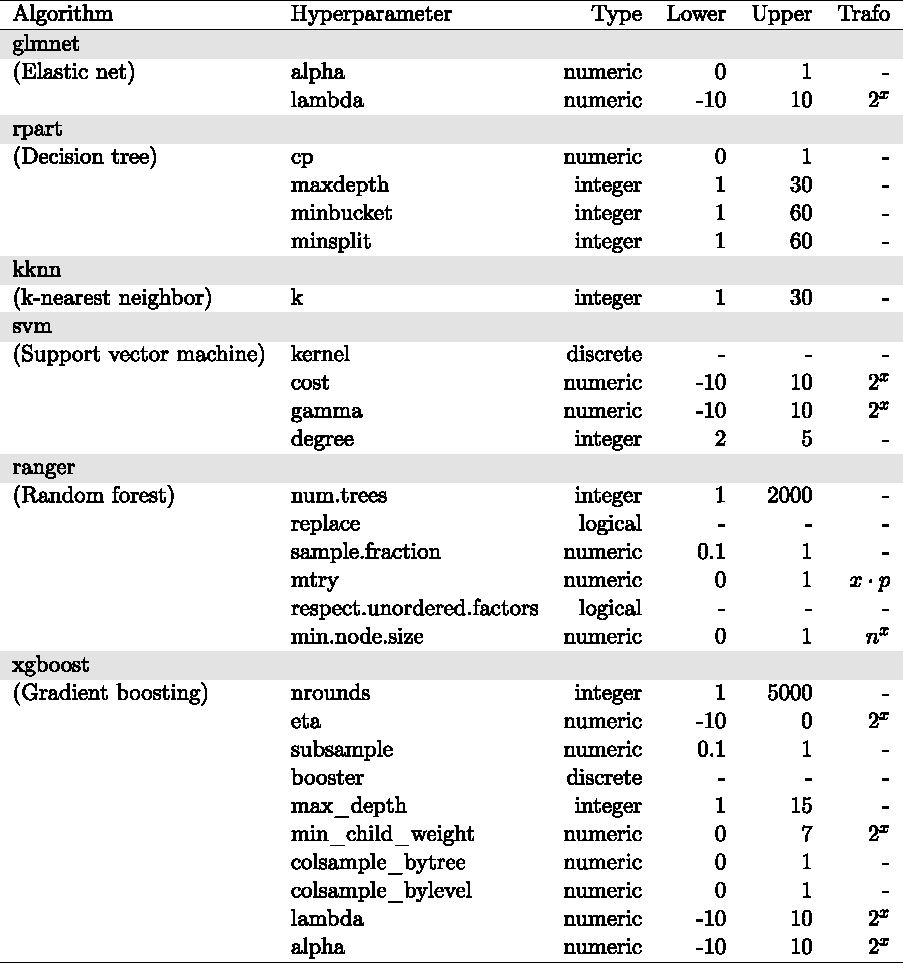
\includegraphics[width = 0.8\linewidth]{images/probst2019jmlr_tab1.pdf}
					{\tiny Source: \lit{\href{https://www.jmlr.org/papers/volume20/18-444/18-444.pdf}{Probst et al. 2019 }}.}
				\end{center}
			\end{column}
			
		  \begin{column}{0.6\textwidth}
		  
		  Ranges often selected based on experience
		  \begin{itemize}
	  
			\item See other AutoML frameworks: e.g.\ Auto-Sklearn~2.0 \lit{\href{https://arxiv.org/pdf/2007.04074.pdf}{Feurer et al. 2020}}
	  
			\item Sensitivity analysis often does not exist for ML~algorithms
			\item Check literature on specific ML algorithm
		  \end{itemize}
		  Options for automation:
		  \begin{enumerate}
			\item Use huge search space to cover all possibilities \\ 
				  (combine with meta-learning for good initial design for Bayesian optimization)
			\begin{itemize} 
					\item Use results of meta-experiments to obtain smaller search space that is estimated to work well.
			 \end{itemize}
			   \item Start with a small space and increase bit by bit
		  \end{enumerate}
		  \end{column}%
	  
		\end{columns}
	  \end{frame}
	  
	  \begin{frame}{Choice of Resampling Strategy}
		
		For computation of generalization error / cost:
		\begin{equation*}
		  \cost(\conf) = \frac{1}{k}\sum_{i = 1}^k \widehat{GE}_{\dataset_{\text{val}}^i}\left(\inducer(\dataset_{\text{train}}^i, \conf)\right)
		\end{equation*}
		% that defines the objective of the black-box optimization we need a resampling strategy.
	  
		\vspace{1em}
		\begin{columns}
		  \begin{column}{0.5\textwidth}
		  Rules of thumb:
		  \begin{itemize}
			\item Default: 10-fold CV ($k=10$)
			\item Huge datasets: holdout
			\item Tiny datasets: 10x10 repeated CV
			\item Stratification for imbalanced classes
		  \end{itemize}
		  \end{column}
		  
		  \begin{column}{0.5\textwidth}
	   Watch out for this:       
		  \begin{itemize}
			\item Small sample size because of imbalances    
			\item Repeated mesurements (leave-one-object out)
			\item Time dependencies
			\item A good AutoML system should let you customize resampling
				% errors here can mean: garbage in, garbvgae out
			\item Meta-learn good resampling strategy~\lit{\href{https://arxiv.org/pdf/2007.04074.pdf}{Feurer et al. 2020}}
		  \end{itemize}
		  \end{column}
		  \end{columns}
		  
	  \end{frame}
	  
	  \begin{frame}{Choice of Optimization Algorithm}
		Choose optimization algorithm based on \ldots
		\begin{itemize}
		  \item complexity of search space / budget
		  \item time-costs of evaluations
		\end{itemize}
	  
		\vspace{0.5em}
	  
		Complex search space
		\begin{itemize}
		  \item[$\rightarrow$] BO with RF surrogate, EA with exploratory character, TPE 
		  % \item[$\rightarrow$] Make use of Grey-Box Optimizers: Hyperband, BOHB
		\end{itemize}
		Numerical (lower-dim) search space and tight budget
		\begin{itemize}
		  \item[$\rightarrow$] BO with GP surrogate\footnote{Still has its own hyperparameters \lit{\href{https://arxiv.org/abs/1908.06674}{Lindauer et al. 2019}}}
		\end{itemize}
		Expensive evaluations
		\begin{itemize}
		  \item[$\rightarrow$] Hyperband, Multi-fidelity BO / EAs, ...
		\end{itemize}
		Deep learning 
		\begin{itemize}
		  \item[$\rightarrow$] common practice: Parameterize architectures, then HPO -- better do it jointly!
		  \item[$\rightarrow$] one-shot models and gradient-based optimization
		\end{itemize}
	  
	\end{frame}

	\begin{frame}{HPO Benchmark Suites}
		\textbf{HPOBench} \lit{{\href{https://openreview.net/forum?id=1k4rJYEwda-}{Eggensperger et al. 2021}}}.
		\begin{itemize}
			\item Successor of HPOlib
			\item Collection of 12 benchmark families; in total $>100$ HPO problems
			\item Mix of tabular, surrogate and real benchmark problems
			\item Also allows for benchmarking multifidelity HPO methods
			\item Benchmarks are containerized making them easily reproducible
		\end{itemize}
		\vspace{1em}
		\textbf{YAHPO Gym} \lit{{\href{https://openreview.net/forum?id=SWcg-TrUgc}{Pfisterer, Schneider et al. 2021}}}.
		\begin{itemize}
			\item Collection of 9 benchmark families constituting over 700 multifidelity multicriteria HPO problems
			\item Surrogate benchmarks using neural-network based instance surrogates
			\item fast inference (< 50 ms) \& low memory footprint ($\sim$ 5 MB)
		\end{itemize}
		\vspace{1em}
		Others: HPO-B \lit{{\href{https://openreview.net/forum?id=O24OhmqpJtP}{Arango et al. 2021}}}.
	\end{frame}
	  


	\begin{frame}{Practical Problems: When to stop?}

		We need to specify a budget, e.g.
		\begin{itemize}
			\item walltime,
			\item function evaluations,
			\item performance threshold, or
			\item \textit{stagnation} for a certain time.
		\end{itemize}

		Problems:
		\begin{itemize}
			\item Overtuning. 
			\item Missed opportunity. 
			\item Wasted computational resources.
		\end{itemize}


		Ways out:
		\begin{itemize}
			\item Early stopping for BO \lit{{\href{https://arxiv.org/abs/2104.08166}{Makarova et al. 2021}}}.
			\item Rules of thumb, maybe $50 \times d$ to $100 \times d$  (\textcolor{red}{be careful and think for yourself!}).
			\item Expert knowledge.
		\end{itemize}

	\end{frame}

	\begin{frame}{Practical Problems: Stability}
		AutoML system should: 
		\begin{itemize}
			\item Never fail to return a result.
			\item Terminate within a given time.
			\item Save intermediate results and allow to continue.
		\end{itemize}

		Failure points:
		\begin{itemize}
			\item Optimizer can crash.
			% $\longrightarrow$ return intermediate result, continue with warmstart / random search
			\item Pipeline training can crash.
			\item Training of a pipeline can run "forever". 
			% \item prediction can crash $\longrightarrow$ use prediction of fallback learner
		\end{itemize}

		Ways out:
		\begin{itemize}
			\item Encapsulate train/predict in separate process from HPO.
			\item Ressource limit time and memory of that process.
			\item If pipeline crashes, run robust fallback (e.g., constant predictor).   
			\item If optimizer proposal crashes, run random configuration.
		\end{itemize}
		
	\end{frame}
	
	\begin{frame}{Practical Problems: Parallelization}
		Parallelization should allow:
		\begin{itemize}
			\item Multiple CPUs/GPUs on a single machine. 
			\item Multiple machines / nodes. 
		\end{itemize}
		
		Possible parallelization levels:
		\begin{itemize}
			\item Training of pipeline.
			\item Resampling.
			\item Evaluation of configurations (batch proposals or asynchronous).
		\end{itemize}
		
		Possible problems:
		\begin{itemize}
			\item Sequential nature of HPO algorithms (e.g.\ BO).
			\item Heterogeneous training times of pipelines can cause idling.
			\item Main memory or CPU-cache becomes bottleneck
			\item Communication between machine / nodes.
		\end{itemize}
	
	Way out: Use a robust framework for parallelization.

	\end{frame}
	
	\begin{frame}{Practical Problems: What to return?}
		What is the output of a an AutoML system, e.g.
		\begin{itemize}
			\item Pipeline with best validation error.
			\item Stacking, e.g. averaging, of top-$k$ pipelines.
			\item Pareto set for multi-objective optimization.
			\item "One-standard-error rule": Use the simplest model within one standard error of the performance of the best model \lit{{\href{https://link.springer.com/book/10.1007/978-0-387-84858-7}{Hastie et al. 2009}}}.
		\end{itemize}
	
		Ensure that simple but efficient pipelines have been tried out 
		\begin{itemize}
			\item Baseline (Classification: Majority vote; Regression: Mean prediction).
			\item Linear Model.
			\item (untuned) Random Forest.
			\item ...
		\end{itemize}
	
	\end{frame}

	\begin{frame}{Interesting Problems}
		\begin{itemize}
			\item How to integrate human a-priori knowledge?
			\item Human-in-the-loop approaches for AutoML.
			\item How can we best (computationally) transfer “experience” into AutoML? 
			\item Warmstarts, learned search spaces, etc.
			\item Multi-Objective goals, including model intepretability and fairness.
			\item AutoML as a process is too much of a black-box, hurts adoption.
			\item Incorporate Uncertainty quantification into AutoML.
			\item AutoML beyond supervised learning.
			\item ...
		\end{itemize}
	
		$\longrightarrow$ Lots of open research questions, feel free to approach us for if you are interested. 

	\end{frame}

\end{document}
